


\begin{frame}[plain,c]
\begin{center}
{\Huge \bf Optional reading for Lecture \thislecture}
\end{center}
\end{frame}

%
%
%

\begin{frame}{Estimating $\int_{a}^{b} \frac{dz}{({\rho}^2+z^2)^{3/2}}$}

We can prove that:
\begin{equation*}
  \int_{a}^{b} \frac{dz}{({\rho}^2+z^2)^{3/2}} = \frac{z}{{\rho}^{2}(z^{2}+{\rho}^{2})^{1/2}} \biggr\rvert_{a}^{b}
\end{equation*}

\vspace{0.2cm}

{\small
One way to calculate this integral is to change variables ($z \rightarrow u$) and perform an integration over the variable u.
A clever variable transformation will leave us with a much simpler integral to calculate.\\

Let's try the following variable transformation:
\begin{equation*}
  z \rightarrow u = tan^{-1}\Big(\frac{z}{{\rho}})\Big)
\end{equation*}

Therefore:
\begin{equation*}
   z = {\rho} tan(u) \;\;\;\; and \;\;\;\;
  dz = {\rho} \Big( tan(u) \Big) du \Rightarrow dz = \frac{{\rho}}{cos^{2}(u)} du
\end{equation*}
}
\end{frame}

%
%
%

\begin{frame}{Estimating $\int_{a}^{b} \frac{dz}{({\rho}^2+z^2)^{3/2}}$}

{\small
With that variable transformation, the integrand becomes:
\begin{equation*}
   \frac{1}{({\rho}^2+z^2)^{3/2}} \rightarrow
     \frac{1}{({\rho}^{2}tan^{2}(u)+{\rho}^{2})^{3/2}} =
     \frac{1}{{\rho}^{3}(tan^{2}(u)+1)^{3/2}} =
     \frac{1}{{\rho}^{3}( \frac{sin^{2}(u)}{cos^{2}(u)}+1)^{3/2}} =
\end{equation*}
\begin{equation*}
   = \frac{1}{{\rho}^{3}( \frac{sin^{2}(u)+cos^{2}(u)}{cos^{2}(u)})^{3/2}} =
     \frac{1}{{\rho}^{3}( \frac{1}{cos^{2}(u)})^{3/2}} =
     \frac{cos^{3}(u)}{{\rho}^{3}}
\end{equation*}

Therefore:
\begin{equation*}
  \int_{a}^{b} \frac{dz}{({\rho}^2+z^2)^{3/2}} =
    \int_{u(a)}^{u(b)} \Big( \frac{cos^{3}(u)}{{\rho}^{3}} \Big) \Big( \frac{{\rho}}{cos^{2}(u)} du \Big) =
    \frac{1}{{\rho}^2} \int_{u(a)}^{u(b)} cos(u) du =
\end{equation*}
\begin{equation*}
   = \frac{1}{{\rho}^2} sin(u) \biggr\rvert_{u(a)}^{u(b)}
   = \frac{1}{{\rho}^2} sin\Big[ tan^{-1}\Big((\frac{z}{{\rho}})\Big) \Big]  \biggr\rvert_{a}^{b}
\end{equation*}
}
\end{frame}

%
%
%

\begin{frame}{Estimating $\int_{a}^{b} \frac{dz}{({\rho}^2+z^2)^{3/2}}$}

\begin{columns}
  \begin{column}{0.30\textwidth}
    {\small
     In order to evaluate the term
     \begin{equation*}
       sin\Big[ tan^{-1}\Big(\frac{z}{\rho}\Big) \Big] \biggr\rvert_{a}^{b}
     \end{equation*}
     appearing in the previous expression,
     consider the triangle below.\\
    }
    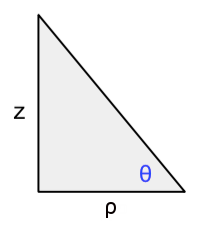
\includegraphics[width=0.85\textwidth]{./images/schematics/triangle_for_integral_in_wire_magnetic_field_calc.png}
  \end{column}
  \begin{column}{0.70\textwidth}
  {\small
    We have:
    \begin{equation*}
      tan(\theta) = \frac{z}{{\rho}} \Rightarrow
      \theta = tan^{-1}\Big( \frac{z}{{\rho}} \Big)  \Rightarrow
      sin(\theta) = sin\Big[ tan^{-1}\Big( \frac{z}{{\rho}} \Big) \Big]
    \end{equation*}
    But:
    \begin{equation*}
      sin(\theta) = \frac{z}{(z^2+{\rho}^2)^{1/2}}
    \end{equation*}
    Therefore:
    \begin{equation*}
       sin\Big[ tan^{-1}\Big( \frac{z}{{\rho}} \Big) \Big] = \frac{z}{(z^2+{\rho}^2)^{1/2}}
    \end{equation*}
    So, indeed, we showed that:
    \begin{equation*}
      \int_{a}^{b} \frac{dz}{({\rho}^2+z^2)^{3/2}} = \frac{z}{{\rho}^{2}(z^{2}+{{\rho}^{2}})^{1/2}} \biggr\rvert_{a}^{b}
    \end{equation*}
  }
  \end{column}
\end{columns}

\end{frame}

% ------------------------------------------------------------------------------
% ------------------------------------------------------------------------------

%
% Programming
%

{
\programmingslide

%
%
%

\begin{frame}{PHYS201 scientific programming task for Lecture \thislecture}

  Background information: {\bf Making a (conventional) neutrino beam}\\

  \begin{columns}
    \begin{column}{0.78\textwidth}
      \centering
      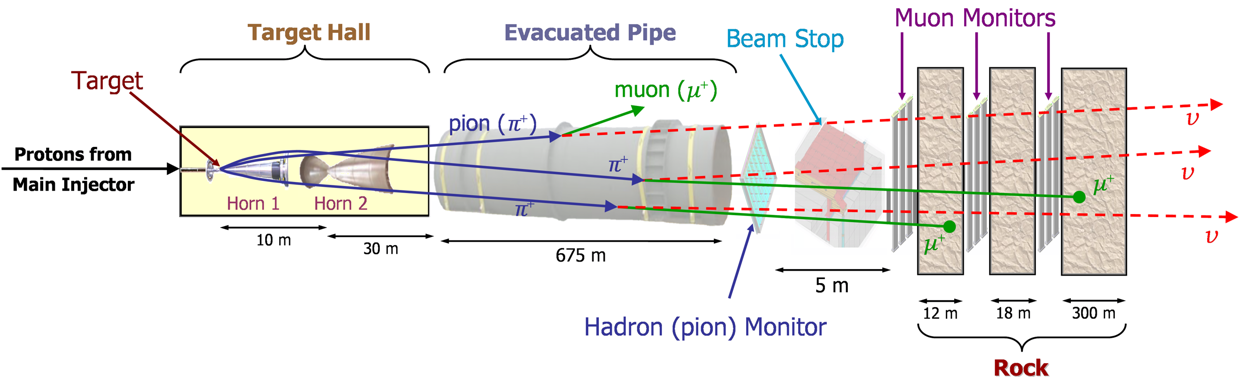
\includegraphics[width=0.95\textwidth]{./images/schematics/numi.png}\\
      \vspace{0.2cm}
      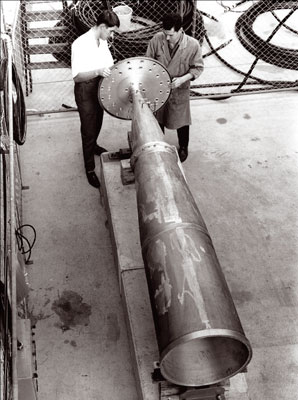
\includegraphics[width=0.32\textwidth]{./images/photos/beam_horn_old_1.jpg}
      \hfill
      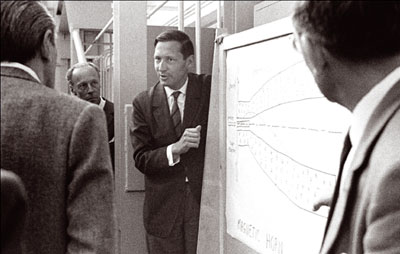
\includegraphics[width=0.66\textwidth]{./images/photos/beam_horn_old_3.jpg}
    \end{column}
    \begin{column}{0.22\textwidth}
     \begin{block}{}
     {\scriptsize
      Where do our $\nu$'s come from?\\
      \vspace{0.3cm}
      $\pi^{+} \rightarrow {\color{red}\nu_{\mu}} + \mu^{+}$\\
      $\pi^{-} \rightarrow {\color{magenta}\bar{\nu}_{\mu}} + \mu^{-}$\\
      $\mu^{+} \rightarrow {\color{magenta}\bar{\nu}_{\mu}} + {\color{blue}\nu_{e}} + e^{+}$\\
      $\mu^{-} \rightarrow {\color{green}\bar{\nu}_{e}} + {\color{red}\nu_{\mu}} + e^{-}$\\
      $K^{+} \rightarrow {\color{red}\nu_{\mu}} + \mu^{+}$\\
      $K^{+} \rightarrow {\color{blue}\nu_{e}} + \pi^{0} + e^{+}$\\
      $K^{+} \rightarrow {\color{red}\nu_{\mu}} + \pi^{0} + \mu^{+}$\\
      $K^{-} \rightarrow {\color{magenta}\bar{\nu}_{\mu}} + \mu^{-}$\\
      $K^{-} \rightarrow {\color{green}\bar{\nu}_{e}} + \pi^{0} + e^{-}$\\
      $K^{-} \rightarrow {\color{magenta}\bar{\nu}_{\mu}} + \pi^{0} + \mu^{-}$\\
      $K_{L}^{0} \rightarrow {\color{magenta}\bar{\nu}_{\mu}} + \pi^{+} + \mu^{-}$\\
      $K_{L}^{0} \rightarrow {\color{red}\nu_{\mu}} + \pi^{-} + \mu^{+}$\\
      $K_{L}^{0} \rightarrow {\color{green}\bar{\nu}_{e}} + \pi^{+} + e^{-}$\\
      $K_{L}^{0} \rightarrow {\color{blue}\nu_{e}} + \pi^{-} + e^{+}$\\
    }
    \end{block}
    \end{column}
  \end{columns}

\end{frame}


%
%
%

\begin{frame}{PHYS201 scientific programming task for Lecture \thislecture}

  Background information: {\bf The hadron hose}\\
  \vspace{0.3cm}
  {\small
  This is an additional {\bf focusing element}.
  It is a wire located in the decay pipe, downstream of the target and
  focussing horns. The wire is pulsed with current creating a toroidal
  magnetic field within the decay volume.\\
  See {\tt \color{blue} J.Hylen et al., https://arxiv.org/pdf/hep-ex/0210051.pdf}\\
  }
  \vspace{0.3cm}
  \begin{center}
    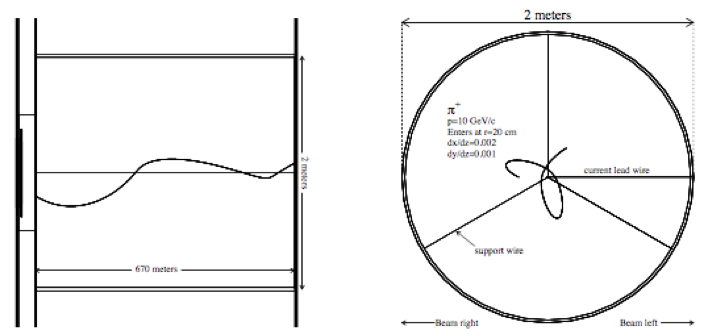
\includegraphics[width=0.75\textwidth]{./images/schematics/hadron_hose_trajectories.png}\\
    {\scriptsize Sample orbit for a 10 GeV $\pi^{+}$.}
  \end{center}
\end{frame}


%
%
%

\begin{frame}{PHYS201 scientific programming task for Lecture \thislecture}

\begin{itemize}
  \item Write a program to {\bf visualise trajectories of charged particles}
        moving in the magnetic field produced by the hadron hose.
  \vspace{0.3cm}
  \item In this lecture, we studied the two main elements for this calculation.
        \begin{itemize}
          \item The magnetic field produced by a long wire.
          \item The magnetic force on a moving electric charge.
        \end{itemize}
  \item The Runge-Kutta method (look it up) can be used for solving the equation
        of motion numerically and calculating the trajectories.
  \vspace{0.3cm}
  \item Assume that the decay pipe has a diameter of 2 m and a length of 700 m.
        Positively-charged pions, with a lifetime of 2.6 $\times$ 10$^{-8}$ $\mu$s
        enter the decay pipe from the centre of its upstream face.\\
        The pions have energies which are uniformly distributed in the 1-5 GeV range,
        and their direction is isotropic in the $\theta$ = $\pm$10$^{o}$ range,
        where $\theta$ is the angle between the hose and the pion direction.\\
        {\bf Optimize the hose current}, so as to maximize the number of pion decays
        within the decay volume and, hence, the neutrino flux.
\end{itemize}

\end{frame}


} % programming


% ------------------------------------------------------------------------------
% ------------------------------------------------------------------------------
